\section{Current state of the Reproducible Builds project}

\subsection[Debian]{Debian}
\nopagebreak[4]{
Debian continues its work towards ensuring that all of the packages in the distribution are bit-by-bit reproducible. 
To continuously check the status of reproducibility of individual packages, testing infrastructure is set up, reporting results on \autocite{tests-rbo}.
For the packages that are not reproducible for the tested variations, the diffoscope output is provided. That allows for an easier identification of underlying issues.\\\\
Currently, the work of Reproducible Builds project members within Debian is focused on three main areas:
\begin{itemize}
\item Continuous testing of Debian packages
\item Categorizing the issues
\item Fixing reproducibility bugs
\end{itemize}
\subsubsection[Continuous testing of Debian packages]{Continuous testing of Debian packages} 
Debian reproducibility testing server \autocite{tests-rbo} shows the status of reproducibility of Debian packages across several releases (stable, unstable, experimental) and architectures (amd64, i386, arm64, armhf). Reproducibility testing here means that the package is built two times, with some variations introduced between builds. For the packages that are not reproducible within this setup, diffoscope is run and its output is published, so it is easily accessible for package maintainers, Reproducible Builds project members and other interested parties. Reproducibility tests are re-run periodically, and the statistics about results of these tests is gathered.\\\\
Figure \ref{fig:stats_sid} shows the current status of reproducibility of Debian packages for unstable version of the distribution built for the amd64 target architecture. Note that the drop in number of reproducible packages in August, 2016 is connected to the new variation -- build path -- being introduced for unstable and experimental distribution. It turned out quite a lot of packages are affected by build path storing issue, and since then, there was quite a lot of work within a project targeting this issue.

\begin{figure}
\centering
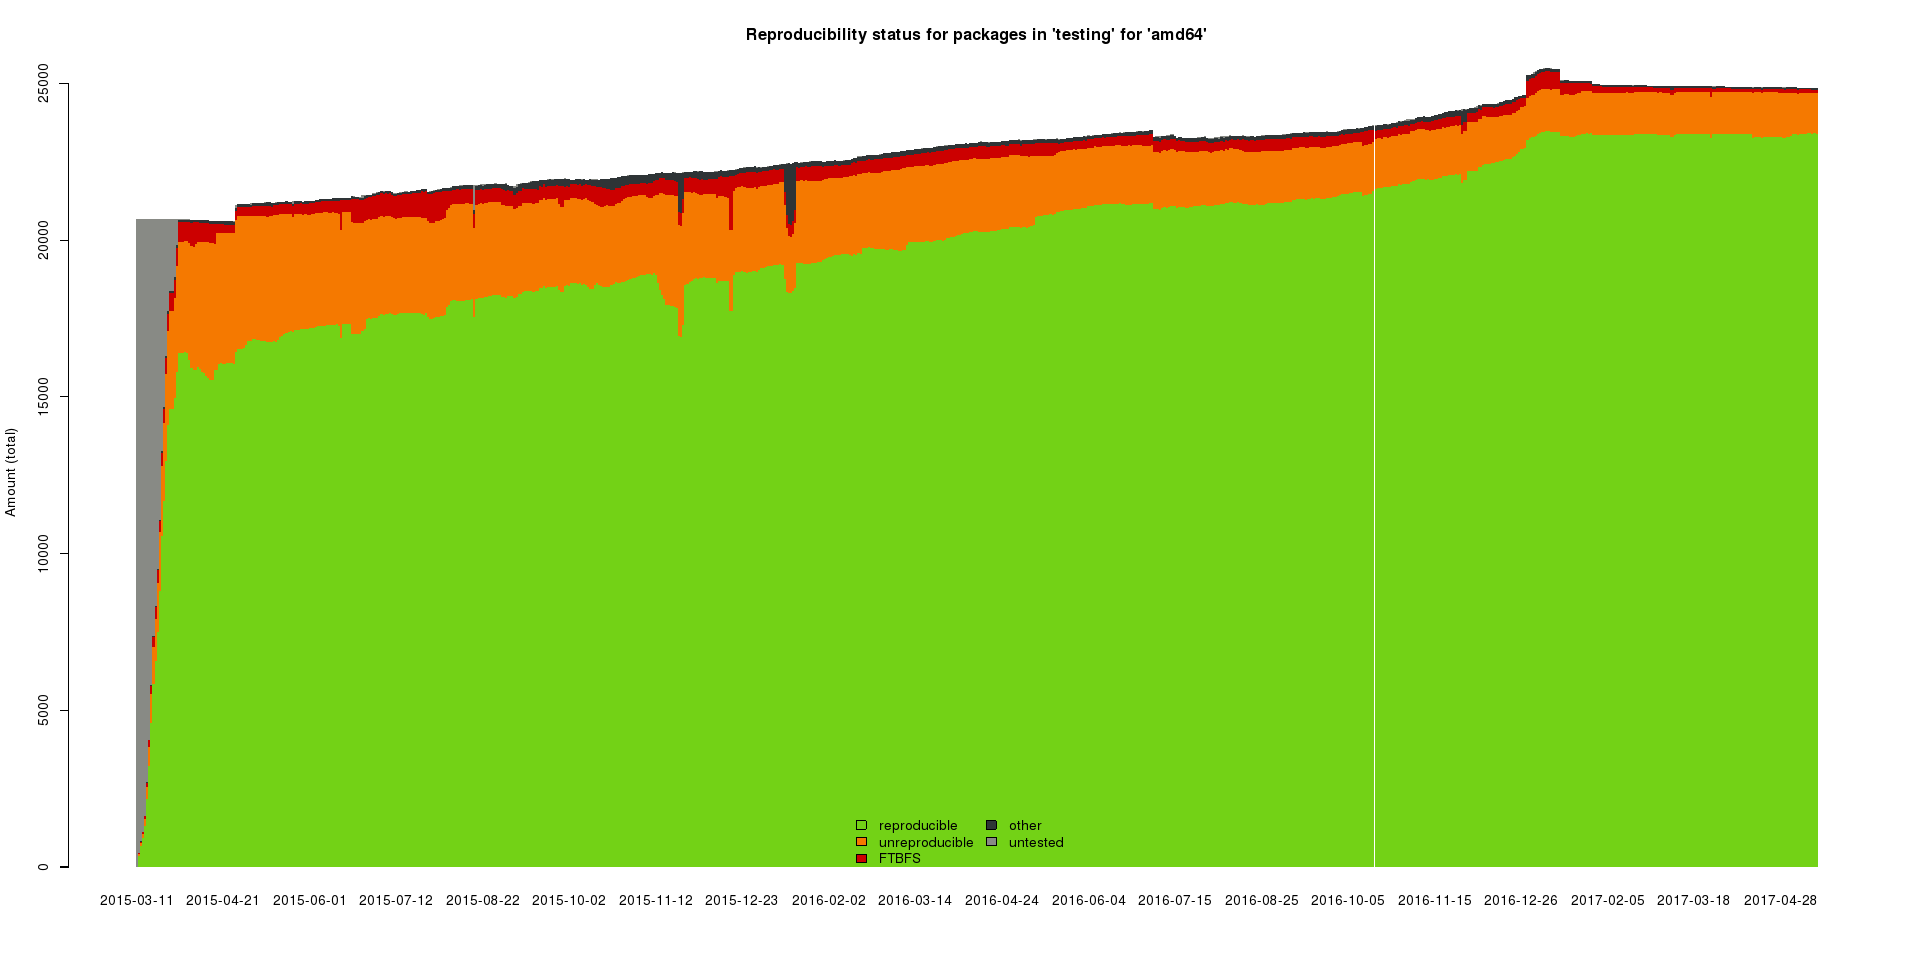
\includegraphics[width=1.0\textwidth]{fig/stats_pkg_state.png}
\caption{\label{fig:stats_sid}Overview of reproducible builds for packages in Debian unstable for amd64 architecture.}
\end{figure}

\subsubsection[Categorizing the issues]{Categorizing the issues} 
With diffoscope result for the packages available, Reproducible Builds project members try to identify the root issue causing reproducibility. It is often the case that the issue is not within the package itself, but rather in the tools used in the build process. Therefore, it is important to identify common issues and focus on resolving them in a unified way.\\\\
Two examples of the most common issues are:
\begin{itemize}[noitemsep]
\item \textit{Capturing build path} -- a lot of packages store the path where the package was built, during the build phase. This is inconvenient since this information is rarely helpful to end users; usually, the package is built on some dedicated build server and not on a target computer. This issue is one of the main focus of Reproducible Build project members now, and they coordinate with the maintainers of packages as well as the build tools developers in order to address it.
\item \textit{Storing Timestamps} -- while this issue was addressed by \texttt{SOURCE\_DATE\_EPOCH}, some packages still record the build date or time.
\end{itemize}
Figure \ref{fig:stats_issues} illustrates the changes in the number of identified issues. This number generally rises over time, as new issues are being found and the old ones are often categorized into smaller and more specific issues. Even if the issue is completely dealt with, it is often left in records if it is believed information about it could be useful to other issues or other projects.\\\\

\begin{figure}
\centering
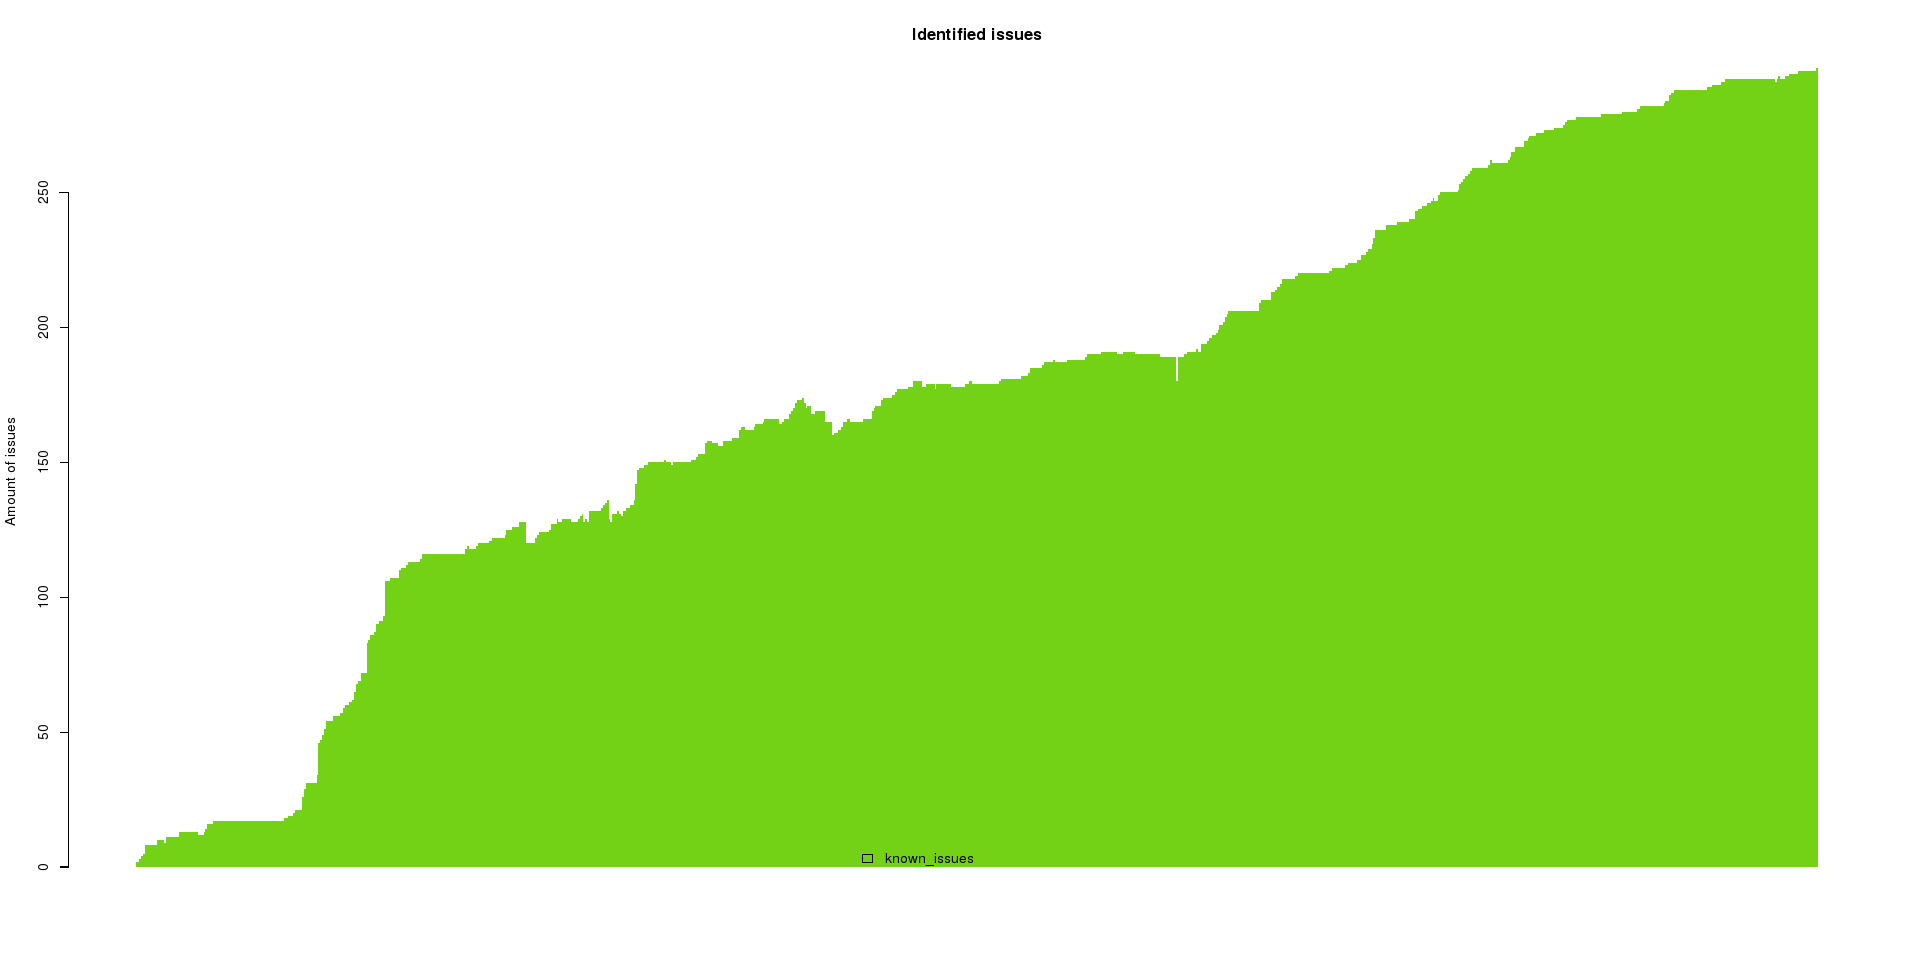
\includegraphics[width=1.0\textwidth]{fig/stats_issues.png}
\caption{\label{fig:stats_issues}Number of categorized reproducibility issues.}
\end{figure}

Figure \ref{fig:stats_notes} shows statistics about number of packages with notes attached to them, meaning that there is an identified issue or some sort of comment for them attached to them. Once again, a massive change is observed at around August, 2016, as the build path variation was introduced, resulting in a lot of packages being labeled with build path recording issue.\\

\begin{figure}
\centering
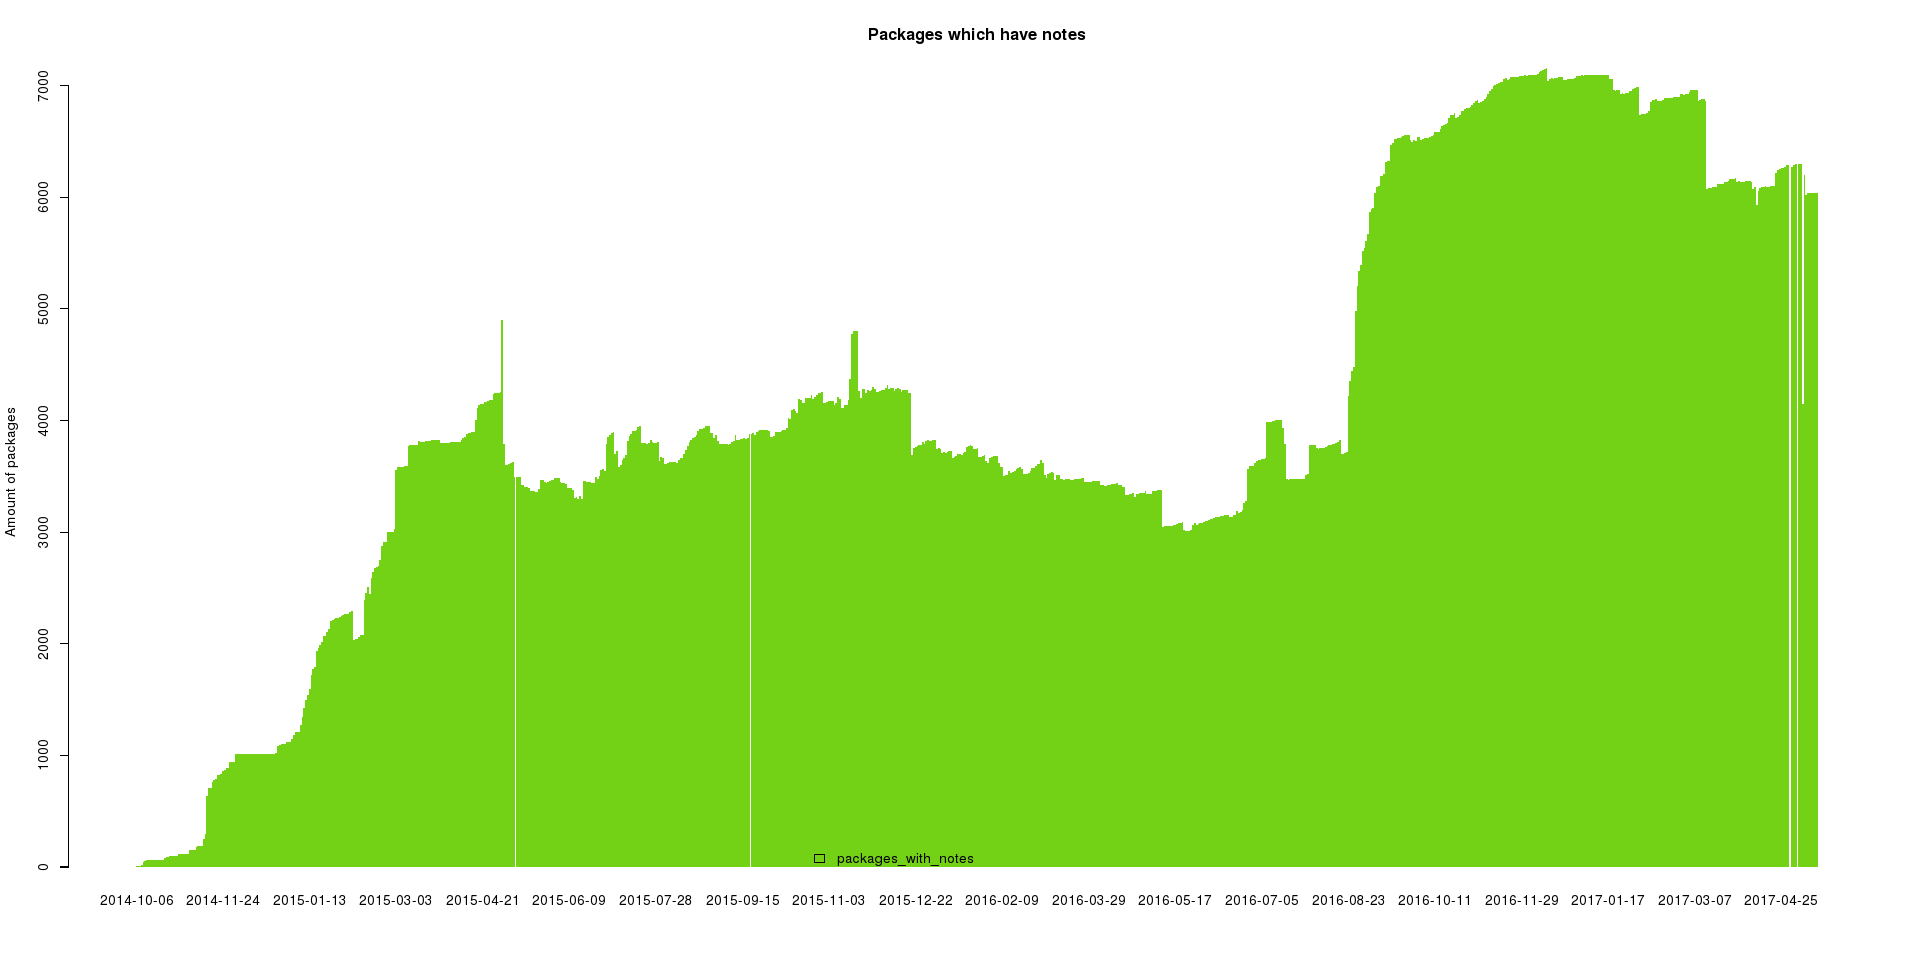
\includegraphics[width=1.0\textwidth]{fig/stats_notes.png}
\caption{\label{fig:stats_notes}Number of packages that have notes.}
\end{figure}
\subsubsection[Fixing reproducibility bugs]{Fixing reproducibility bugs}
While only package maintainers or developers actually have the means to fix their package, members of Reproducible Builds project try to help them by reporting the reproducibility issue. As a rule, they also provide a patch that is expected to fix the issue. Sometimes additional coordination with package maintainer or developer is required to ensure the patch fits well within the package and to clarify its meaning.\\\\
A lot of issues are related to the usage of the specific tool in the build process, and therefore it is usually preferred to focus on fixing these issues in the build tool in question, therefore helping all the packages using that tool to achieve reproducibility.

}
\subsection[F-droid]{F-droid}
\nopagebreak[4]{
The F-Droid project \autocite{fdroid}, that aims to provide an environment of free software for Android smartphones, has set up its own Verification Server \autocite{fdroid-vfs}. It functions in the similar fashion as Debian test infrastructure, rebuilding packages and providing the diffoscope output when results do not match.\\
}
\subsection[Other projects]{Other projects}
\nopagebreak[4]{
FreeBSD and NetBSD distributions also continue their work on reproducible builds. Currently, they use less variations between builds than Debian does, but within these constraint, they have achieved significant progress: NetBSD reported 100\% reproducibility within their build system in \autocite{netBSD} and FreeBSD is at 99.6\% at the moment \autocite{freeBSD}.
}


%\cleardoublepage
